\chapter{Systementwurf}
\label{ch:Design}

Ein wichtiger Teil dieser Arbeit ist die Erstellung eines Datensatzes, welcher zur Klassifikation dienen soll.
Mithilfe einer Smartphone-App soll ein Datensatz eines Studienteilnehmers erstellt und exportiert werden. 
Daraufhin liegen die Daten vor und können in einer Verarbeitungspipeline analysiert, beziehungsweise klassifiziert werden.

Die Studie wurde so konzipiert, Atemaussetzer während des Schlafens zu klassifizieren. 
Während der Studie wurde jeder Datensatz im Bett des Teilnehmers aufgezeichnet, was das Wohlbefinden verstärken und somit auch die Qualität der Daten erhöhen soll.

%Dadurch, dass bei der Studie neben den eSense Earpods auch ein PSG-System zum Sammeln der Daten benutzt wird, gestaltet sich die Suche nach Probanden als sehr schwer. 
%Das PSG-System sammelt medizinische Daten, welche nicht ohne Antrag bei der Ethikkommission (REC, \textit{resarch ethics committee}) erhoben werden dürfen. 
Im Rahmen dieser Bachelorarbeit wurde ein Datensatz  nach dem \textit{Sample of Convenience} erstellt.

\section{Studienplanung}
\label{ch:Design:sec:studienplanung}
Für die Studie wurde pro Teilnehmer ein Datensatz an 3 verschiedenen Positionen aufgezeichnet, auf dem Bauch, dem Rücken, sowie auf der Seite liegend.

Eine Fragestellung der Studie war, wie ein Atemaussetzer {\glqq simuliert\grqq} werden soll. 
Es wurde entschieden, dass die Studie eine zentrale Schlafapnoe erkennen soll. 
Demzufolge soll der Studienteilnehmer in einer vordefinierten Reihenfolge einen Atemaussetzer {\glqq simulieren\grqq}, indem er die Luft für eine gewisse Zeit anhält.
Um unterschiedliche Längen von Atemaussetzern aufzuzeichnen, wurde eine Länge von $10\si{\s}$, $20\si{\s}$ und $30\si{\s}$ gewählt, in welchen der Teilnehmer die Luft anhalten soll. 
Nun muss ein geeigneter Ablauf gewählt werden, wodurch sich die Ereignisse nicht überschneiden.
Auf der Suche, wie lange die Regeneration dauere, nachdem eine Person die Luft angehalten hat, ergab sich durch das Schaubild \ref{fig_respiration_regeneration}, dass die Person circa die gleiche Zeit zur Regeneration benötigt, wie sie die Luft zuvor angehalten hat.
Diese Zeit wurde mit etwas Puffer nun zusätlich in der Studie mit eingebracht und daraus ergibt sich der Ablauf, welcher in Abbildung \ref{fig_study_flow} zu sehen ist.

\begin{figure}[ht]
    \centering
    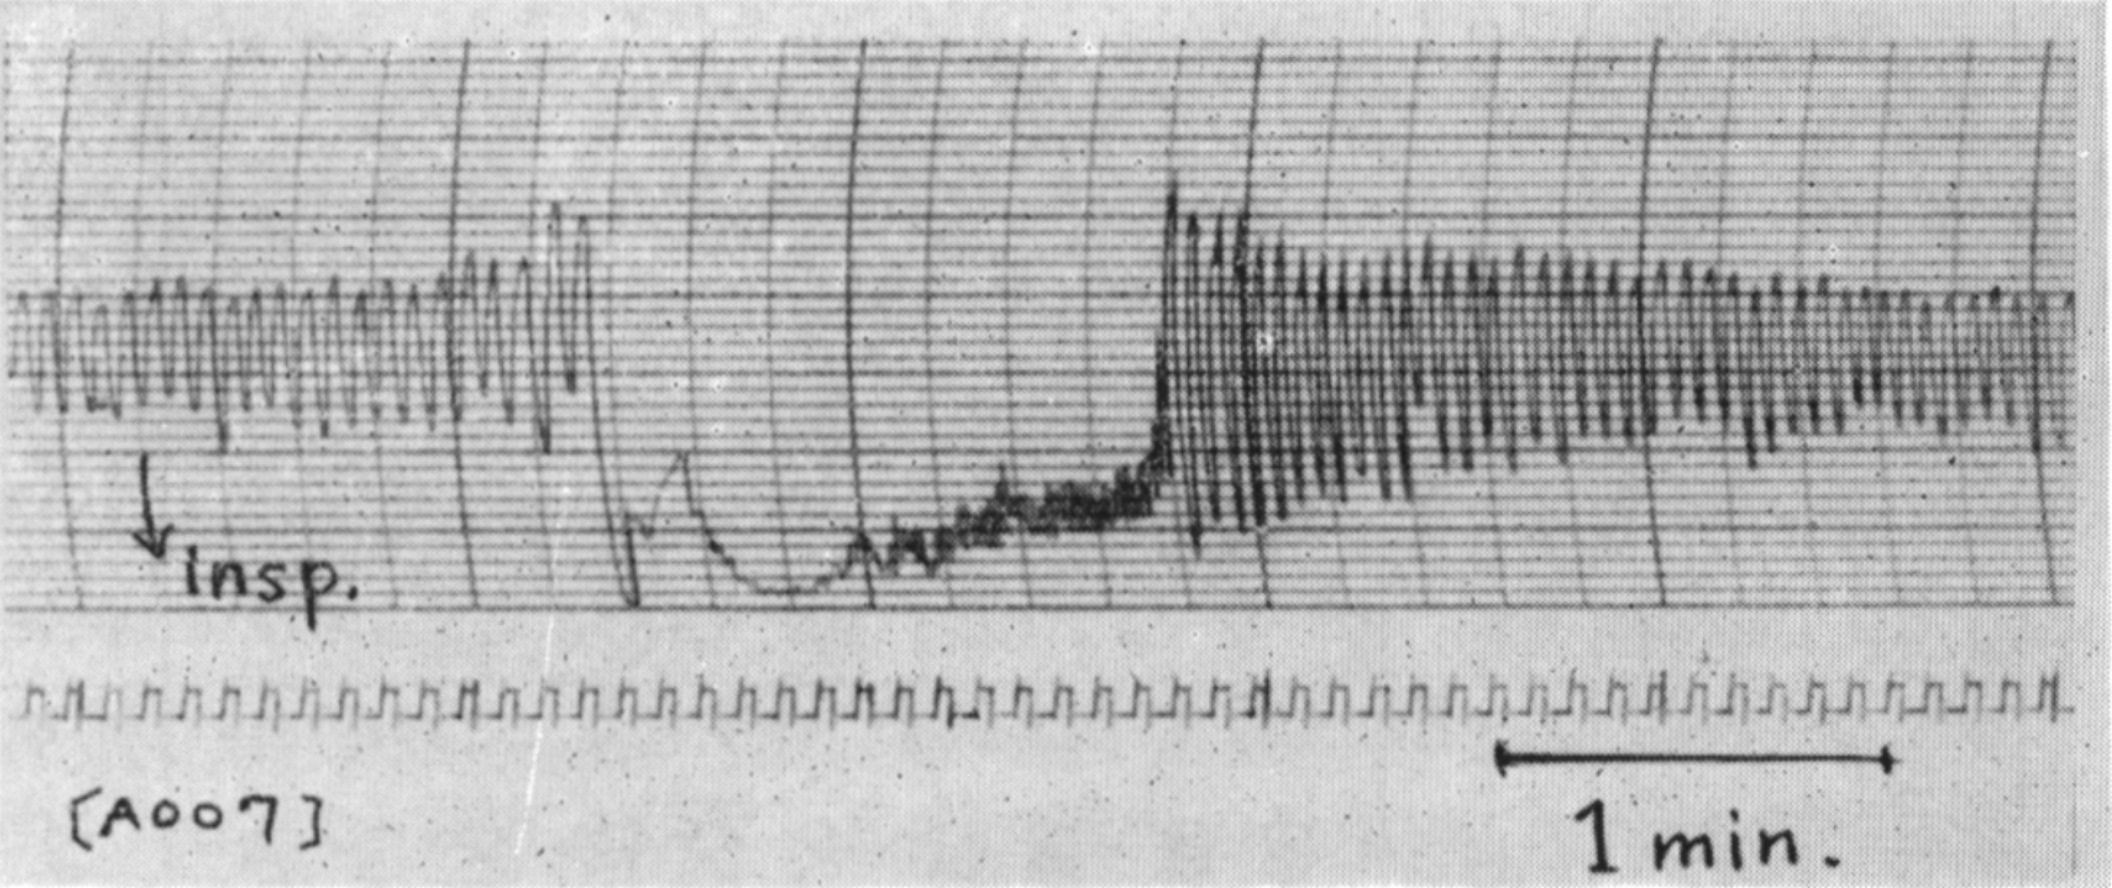
\includegraphics[width=0.66\textwidth]{images/respiration/respiration_regeneration}
    \caption{Regenerationsphase nach dem Luftanhalten \cite{beath_rebreathing}.}
    \label{fig_respiration_regeneration}
\end{figure}

\begin{figure}[ht]
    \centering
    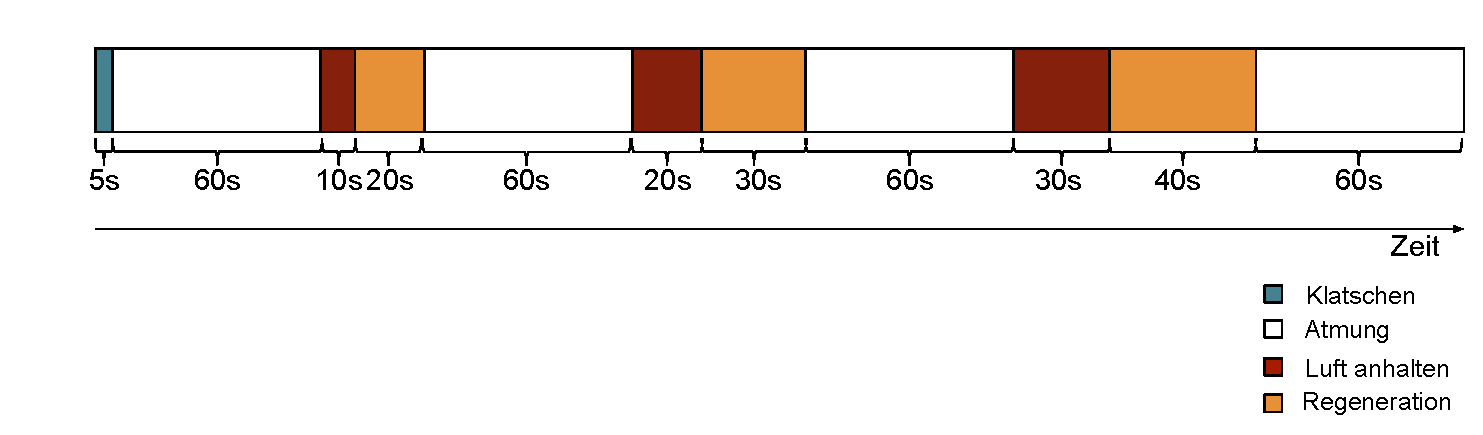
\includegraphics[width=1\textwidth]{images/study/study_flow2}
    \caption{Ablauf der Studie mit einer Position}
    \label{fig_study_flow}
\end{figure}


\section{Systemmodelle}
Zur Datenaufzeichnung während der Studie wurde eine Smartphone-App für Apple-Geräte konzipiert und mit der Sprache Swift entwickelt. 
Mit der Software XCode lässt sich eine mit Swift geschriebene App kompilieren und auf dem Smartphone installieren.

Zur Einbindung externer Frameworks werden die Dependency-Manager \textit{Accio} und \textit{Carthage} verwendet.
Im Folgenden sind die relevanten Frameworks aufgelistet, welche in der App eingebunden worden sind:

\begin{center}
  \begin{tabular}{ | l | l | }
    \hline
    Imperio & Strukturierung der App \\ \hline
    Realm-Cocoa & Datenbank-Framework \\ \hline
    Zip & Bietet die Möglichkeit, einen Ordner \\ 
    & als {\glqq zip\grqq}-Datei zu komprimieren\\ \hline
    Mungohealer & Fügt Logging zu der App hinzu \\
    \hline
  \end{tabular}
\end{center}

Durch das Framework \textit{Imperio} ist es möglich, die View-Komponenten von der Logik zu trennen. 
Somit ändert sich die Struktur der App, indem jeder Ablauf in der App als \textit{Flow} interpretiert wird. 
Pro Flow wird ein \textit{FlowController} angelegt, welcher die Logik des Ablaufs kontrolliert. 
Ein Flow kann nun beliebig viele \textit{ViewController} starten.
Jede \textit{View}, welche von einem Flow aufgerufen wird, hält ein \textit{Delegate} Objekt.
Ein \textit{Delegate} ist ein Protokoll, womit dem \textit{Flow} eine Aktion auf der \textit{View} mitgeteilt werden kann.
Somit wird bei jeder Aktion auf der View eine Funktion des FlowControllers aufgerufen, welcher die View gestartet hat.

\todo{grafik hinzufügen (einfache Grafik anscheinend)}

Das Framework \textit{Realm} ist eine Datenbank für mobile Systeme, die vollständig auf dem mobilen Endgerät läuft.
Die Daten können direkt als \textit{Objekt} ausgelesen und verarbeitet werden.
In der App wird die Datenbank verwendet, um eine Messung abzuspeichern (siehe Abbildung \ref{implementation:app:erModel}))

Das Framework \textit{Mungohealer} stellt eine Möglichkeit dar, bessere Fehlerbenachrichtigungen erstellen zu können. 
Der Standard, welcher von Apple bereitgestellt wird (\textit{NSERROR}), wird durch dieses Framework erweitert.
Somit können Fehler in der Konsole genauer beschrieben werden. 
In dieser App wird dies unter anderem verwendet, um Benachrichtigungen der Bluetoothverbindung zu den eSense-Earpods zu erhalten.